% !TeX spellcheck = de_AT_frami
\documentclass[10pt,a4paper]{article}
\usepackage[utf8x]{inputenc}
\usepackage[naustrian]{babel}
\usepackage{ucs}
\usepackage{amsmath}
\usepackage{amsfonts}
\usepackage{amssymb}
\usepackage{bm}
\usepackage{graphicx}
\usepackage{txfonts}
\usepackage[dvipsnames]{xcolor}
\usepackage{geometry}
\usepackage{graphicx}
\usepackage{epstopdf}
\epstopdfsetup{update}
\geometry{margin= 2cm}
\usepackage{multirow}
\usepackage{cellspace}
\usepackage[hidelinks]{hyperref}
\usepackage[mathscr]{euscript}
\usepackage{commath}

\usepackage{scalerel,stackengine}
\stackMath
\newcommand\reallywidehat[1]{%
	\savestack{\tmpbox}{\stretchto{%
			\scaleto{%
				\scalerel*[\widthof{\ensuremath{#1}}]{\kern-.6pt\bigwedge\kern-.6pt}%
				{\rule[-\textheight/2]{1ex}{\textheight}}%WIDTH-LIMITED BIG WEDGE
			}{\textheight}% 
		}{0.5ex}}%
	\stackon[1pt]{#1}{\tmpbox}%
}
\parskip 1ex



\setlength\parindent{0pt}
\renewcommand*{\theenumi}{\thesection.\arabic{enumi}}
\renewcommand*{\theenumii}{\theenumi.\arabic{enumii}}

\begin{document}
	\pagenumbering{gobble}
	\title{
		\mbox{}
		\vspace{5cm} \\
		VO Numerische Mathematik
		\\
		2017/18
		\\
		Theoriefragen \\
		\vspace{\fill}
		\large\url{https://github.com/Arkonos/NM_Theorie_1718}
	}
	\maketitle
	
	\newpage
	% !TeX spellcheck = de_AT_frami
\section{Zahldarstellung, Rundung und Fehler}
	\begin{enumerate}
		\item \textbf{Wie werden ganze Zahlen binär abgespeichert?}\\
			S. 2
			\begin{align*}
				b_{N-1}b_{N-2}\dots b_{1}b_{0} \cong b = \sum_{j=0}^{N-1}b_j2^j, \quad b_j\in\{0,1\}
			\end{align*}
			Beispiel: \(23_{10}\)
			\begin{align*}
					10101_2 &= 1\cdot2^4+0\cdot2^3+0\cdot2^2+1\cdot2^1+1\cdot2^0 \\
					      &= 16+0+0+2+1 = 19_{10}
			\end{align*} \vspace{-1cm}
			\begin{figure}[htbp]
				\centering
				\begin{minipage}{0.3\textwidth}
					\centering
					$$\begin{array}{rrrrrr}
					\multirow{2}{*}{:2} & 19 & 9 & 4 & 2 & 1 \\
					\cline{2-6}
					 \rule{0pt}{2.5ex} & 1 &  1 & 0 & 0 & 1
					\end{array}$$
				\end{minipage}\hspace{-0.5cm}
				\begin{minipage}{0.01\textwidth}
					\centering
					\vspace{0.3cm}
					\(\rightarrow\)
				\end{minipage}\hspace{-0.7cm}
				\begin{minipage}{0.2\textwidth}
					\centering
					\vspace{0.3cm}
					\(10011_2\)
				\end{minipage}
			\end{figure}
			
			
		\item \textbf{Wie werden Gleitpunktzahlen (doppelte Genauigkeit) binär abgespeichert?}\\
		S. 3
			\begin{align*}
				x &= (-1)^s \cdot m \cdot 2^e \\
				x &\cong s \;\;\; e_{11}e_{10}\dots e_0 \;\;\; (m_0).m_1m_2\dots m_{51}
			\end{align*}\vspace{-0.5cm}
			\begin{table}[htbp]
				\centering
				\begin{tabular}[htpb]{rll}
					s \; \dots \!\!\! & Vorzeichenbit &\(\in \{0,1\}\)\\
					m \; \dots \!\!\! & Mantisse & Normiert, \(m_0\overset{!}{=}1\) wird weggelassen\\
					e \; \dots \!\!\! & Exponent & nach Abzug von b\(\dots\)Bias = 1023 (double)
				\end{tabular} \\ \vspace{0.3cm}
				\begin{tabular}[htpb]{rccc}
					 & s & m & l \\
					  single 32 Bit & 1 & 23 & 8 \\
					  double 64 Bit & 1 & 52 & 11
				\end{tabular}
			\end{table}
		\item \textbf{Wie werden Gleitpunktzahlen gerundet?} \\
		S. 6 \\
		Round to the nearest even.
		\begin{table}[htbp]
			\centering
			\begin{tabular}[htpb]{ccccccl}
				\dots & \(\text{m}_\text{M}\) & \(\text{m}_{\text{M}+1}\) & \(\text{m}_{\text{M}+2}\) & \(m_{M+3}\) & \dots &  \\
				      & x                   & 0                       & x                       & x         &       & abrunden  \\
				      & x                   & 1                       & 1                       & 0         &       & aufrunden \\
				      & x                   & 1                       & 0                       & 1         &       & aufrunden \\
				      & 1                   & 1                       & 0                       & 0         &       & aufrunden \\
				      & 0                   & 1                       & 0                       & 0         &       & abrunden
			\end{tabular}
		\end{table}
		\item \textbf{Wie ist der relative Rundungsfehler definiert?} \\
		S. 6
		\begin{align*}
			\frac{\abs{\text{rd}(x)-x}}{\abs{x}}\leq \frac{2^{-\text{M}-1}\cdot2^e}{\text{a}\cdot 2^e}\underset{\text{a}\in[1,2)}{\leq}2^{-\text{M}-1}=:\texttt{eps} \\
			\text{rd}(a) \text{ durch rounding to the nearest even} 
		\end{align*}
		
		\item \textbf{Wie groß ist die relative Maschinengenauigkeit \texttt{eps} für doppelt genaue Gleitpunktzahlen?\\
					Wie kann man \texttt{eps} experimentell bestimmen?} \\
				
				
		\item \textbf{Was ist die relative/absolute Kondition eines Problems?}
			\begin{align*}
				\frac{\abs{f(\tilde{x})-f(x)}}{\abs{f(x)}} &\leq \kappa_{\text{rel.}}\cdot\varepsilon, \quad \kappa_{\text{rel.}} > 0 \\
				\abs{f(\tilde{x})-f(x)} &\leq \kappa_{\text{abs.}}\cdot\delta, \quad \kappa_{\text{abs.}} > 0
			\end{align*}
		Wenn \(\kappa_{\text{rel.}}\) klein ist werden Inputfehler nicht übermäßig verstärkt und \(f\) gilt als gut konditioniert.
		\item \textbf{Was bedeuten die Begriffe Konsistenz und Konsistenzordnung?} \\
			Def 1.3 Konsistenz, Konsistenzordnung \\
			Ein numerisches Verfahren \(f_h\) mit Diskretisierungsweite h zur Bestimmung einer Näherung von \(f_h(x)\) an \(f(x)\) ist konsistent, falls gilt
			\begin{align*}
				\norm{f_h(x)-f(x)}\leq \text{C}\,h^\text{p}
			\end{align*}
			wobei die Konstante \(\text{C}>0\) nicht von h abhängen darf und \(p\ge1\). Der Exponent \(p\) ist dann die Konsistenzordnung und es gilt \(f_h\rightarrow f\) für \( h \rightarrow 0\), falls \(f_h\) exakt ausgewertet wird. 
		
		\item \textbf{Wodurch unterscheidet sich Konsistenz von Konvergenz?} \\
			\(f_h\rightarrow f\) konvergiert für \( h \rightarrow 0\) falls \(f_h\) exakt ausgewertet wird. Computer müssen jedoch runden, wodurch wir nur noch von Konsistenz reden können wenn das Verfahren nicht stabil ist.
		
		\item \textbf{Was bedeutet der Begriff Stabilität?} \\
		S. 15\\
		Ein numerisches Verfahren \(f\) heißt stabil, falls bei der numerischen Auswertung \(\tilde{f}(x)\) des Verfahrens Fehler wie Rundungsfehler, Abbruchfehler und Verfahrensfehler von Teilschritten nicht	übermäßig verstärkt werden im Vergleich zu dem durch die relative Kondition \(\kappa_{rel}\) des Problems verursachten Fehler. \\
		Für die Differenz zwischen numerischer Auswertung \(\tilde{f}(x)\) mit obigen Fehlern und exakter Auswertung \(f(x)\) gilt dann
		\begin{align*}
			\norm{\tilde{f}(x)-f(x)}\leq \text{C}\cdot\kappa_{rel.}\cdot\abs{f(x)}\cdot\texttt{eps}, \quad \text{C} > 0 \text{ klein.}
		\end{align*}
		Ein numerisches Verfahren ist insbesondere dann stabil, wenn alle seine Teilschritte gut konditioniert sind.
		
	\end{enumerate}
	\newpage
	\section{Numerische Differentiation}
	\begin{enumerate}
		\item \textbf{Wie wird mit Hilfe der Vorwärtsdifferenz eine differenzierbare Funktion $\pmb{f}$ an der Stelle $\pmb{x}$ differenziert? Wie groß ist $\pmb{h_{opt}}$?}\\
		
		\item \textbf{Wie wird mit Hilfe der zentralen Differenz eine differenzierbare Funktion $\pmb{f}$ an der Stelle $\pmb{x}$ differenziert? Wie groß ist $\pmb{h_{opt}}$}\\
		\item \textbf{Wie verhalten sich Verfahrensfehler und Rundungsfehler in Abhängigkeit von der Schrittweite $\pmb{h}$? Machen Sie eine Skizze.}\\
		\item \textbf{Wie lässt sich mit Hilfe eines logarithmischen Plots das Verhalten von Verfahrensfehler und Rundungsfehler ablesen? Wie kann man die optimale Schrittweite $\pmb{h_{opt}}$ ablesen?}\\
		\item \textbf{Wieso gilt bei der zentralen Differenz für den Verfahrensfehler $\pmb{V(h)=\mathcal{O}(h^2)}$ statt $\pmb{\mathcal{O}(h)}$?}\\
		\item \textbf{Wie wird die zweite Ableitung einer zweimal differenzierbaren Funktion an der Stelle $\pmb{x}$ berechnet? Wie groß ist $\pmb{h_{opt}}$?}\\
		\item \textbf{Wie lässt sich die optimale Schrittweite $\pmb{h_{opt}}$ aus dem Verfahrensfehler $\pmb{V(h)}$ und dem Rundungsfehler $\pmb{R(h)}$ bestimmen?}\\
		\item \textbf{Wie berechnet man die Jacobimatrix einer vektorwertigen Funktion $\pmb{f:}{\rm I\!R}\pmb{^n} \rightarrow {\rm I\!R}\pmb{^m}$ durch numerisches Differenzieren?}\\
		\item \textbf{Wie berechnet man den Gradient einer skalaren Funktion $\pmb{f:}{\rm I\!R}\pmb{^n} \rightarrow {\rm I\!R}\pmb{^m}$ durch numerisches Differenzieren?}\\
	\end{enumerate}
	\newpage
	% !TeX spellcheck = de_AT_frami
\section{Interpolation}
	\begin{enumerate}
		\item \textbf{Wie werden die dividierten Differenzen berechnet?} \\
			Mit Hilfe eines Differenzenschema oder Differenzentableau. \\
			Allgemeines Differenzenschema für 5 Punkte
				\begin{align*}
				\begin{array}{cc|cccc}
					x_i & y_i &              \delta y_i              &                     \delta^2 y_i                     &                       \delta^3 y_i                       &                       \delta^4 y_i                       \\ \hline
					x_0 & y_0 &  \\
					    &     & \delta y_0 = \frac{y_1-y_0}{x_1-x_0} &  \\
					x_1 & y_1 &                                      & \delta^2 y_0 = \frac{\delta y_1-\delta y_0}{x_2-x_0} &  \\
					    &     & \delta y_1 = \frac{y_2-y_1}{x_2-x_1} &                                                      & \delta^3 y_0 = \frac{\delta^2 y_1-\delta^2 y_0}{x_3-x_0} &  \\
					x_2 & y_2 &                                      & \delta^2 y_1 = \frac{\delta y_2-\delta y_1}{x_3-x_1} &                                                          & \delta^4 y_0 = \frac{\delta^3 y_1-\delta^2 y_0}{x_4-x_0} \\
					    &     & \delta y_2 = \frac{y_3-y_2}{x_3-x_2} &                                                      & \delta^3 y_1 = \frac{\delta^2 y_2-\delta^2 y_1}{x_4-x_1} &  \\
					x_3 & y_3 &                                      & \delta^2 y_2 = \frac{\delta y_3-\delta y_2}{x_4-x_2} &  \\
					    &     & \delta y_3 = \frac{y_4-y_3}{x_4-x_3} &  \\
					x_4 & y_4 &
				\end{array}
			\end{align*}
		\item \textbf{Wie ist das Newtonsche Interpolationspolynom definiert?}
			\begin{align*}
				p(x)=y_0+(x-x_0)\delta y_0+(x-x_0)(x-x_1)\delta^2 y_0+\dots+(x-x_0)(x-x_1)\cdots(x-x_{n-1}) \delta^\text{n} y_0
			\end{align*}
		
		\item \textbf{Wie wird mit dem Hornerschema ein Polynom $\mathbf{p(x)=a_0+a_1x+\dots +a_nx^n}$ ausgewertet?} \\
			\begin{align*}
				p(x)=a_0+x(a_1+x(a_2+\cdots+x(a_{n-2}+x(a_{n-1}+x\,a_n))\cdots))
			\end{align*}
		\item \textbf{Wie wird mit dem Hornerschema ein Newtonsches Interpolationspolynom ausgewertet?}
			\begin{figure}[htbp]
				\centering
				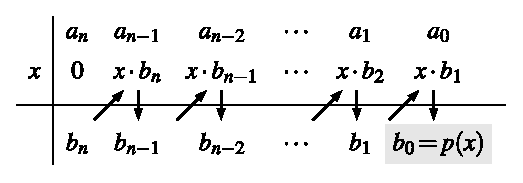
\includegraphics[width=0.45\linewidth]{Kap3_1}
			\end{figure}
		\item \textbf{Wie sind die Lagrange-Polynome definiert? Welche Eigenschaften haben sie?}
			\begin{align*}
				\ell_i(x)&=\frac{(x-x_0)(x-x_1)\cdots\reallywidehat{(x-x_i)}\cdots(x-x_n)}{(x_i-x_0)(x_i-x_1)\cdots\reallywidehat{(x_i-x_i)}\cdots(x_i-x_n)} \\
				\ell_i(x_j)&=\delta_{ij} =
					\begin{cases}
						1, & \text{falls } i=j,\\
						0, & \text{falls } i\neq j.
					\end{cases} \nonumber
			\end{align*}
			Wobei die überdachten Terme wegzulassen sind.
		\item \textbf{Wie wird mit Hilfe der Lagrange-Polynome das Langrangesche Interpolationspolynom berechnet?}
			\begin{align*}
				p(x)=\sum_{i=0}^{n}y_i\,\ell_i(x), \quad p(x_j)=y_j
			\end{align*}
		
		\item \textbf{Erklären Sie die Begriffe Datenfehler, Verstärkungsfaktor, Lebesgue-Funktion und Lebesgue-Konstante in Zusammenhang mit der Polynominterpolation. Was ist die Kondition der Polynominterpolation?} \\
			An einer Stützstelle \(x_j\) kann ein Datenfehler \(\varepsilon_j\) auftreten.
			Führt man diesen in ein Lagrange-Polynom ein erhält man
			\begin{align*}
				\overline{p}(x)=\sum_{i=0}^{j-1}\left( y_i\,\ell_i(x)\right) + (y_j+\varepsilon_j)+\sum_{i=j+1}^{n}\left( y_i\,\ell_i(x)\right).
			\end{align*}
			Der Fehler \(\varepsilon_i\) wird also um den Faktor \(|\ell_i|\) verstärkt.
			Wenn alle Knoten mit Fehlern verseht sind ergibt sich
			\begin{align*}
				\overline{p}(x)=p(x)+\sum_{i=0}^{n}\left( \varepsilon_i\,\ell_i \right) .
			\end{align*}
			Falls die einzelnen Fehler durch \(\varepsilon_i\le\text{M}\) beschränkt sind erhält man für den absoluten Fehler die Abschätzung
			\begin{align*}
				\underbrace{|\overline{p}(x)-p(x)|}_\text{abs. Fehler Output}\leq \text{M}\underbrace{\sum_{i=0}^{n}\overbrace{|\ell_i(x)|}^{\kappa_{\text{abs},i}(x)}}_{\kappa_\text{abs}(x)}
				= \text{M}\cdot\kappa_\text{abs}(x).
			\end{align*}
			Wobei \(\kappa_{\text{abs},i}=|\ell_i(x)|\) der Verstärkungsfaktor für den Datenfehler in der Stützstelle \(i\) und die Lebesgue-Funktion \(\kappa_\text{abs}=\lambda_n(x)=\sum_{i=0}^{n}|\ell_i(x)|\) die absolute Kondition für die Polynominterpolation ist. Die schlechteste Konditionszahl \(\lambda_n(x)\) im Intervall \([\text{min}_ix_i,\text{max}_ix_i]\) nennen wir Lebesgue-Konstante und erhalten sie durch
			\begin{align*}
				\underset{x\in[\text{min}_ix_i,\text{max}_ix_i]}{\text{max}} \lambda_n(x):=\Lambda_n.
			\end{align*}
		\item \textbf{Was besagt der Satz über den Fehler des Interpolationspolynoms? Wie ist der Verfahrensfehler definiert?} \\
		
		\item \textbf{Wie sind die Tschebyscheff-Polynome definiert? Welche Eigenschaften haben sie?} \\
		
		\item \textbf{Wie berechnet man die Knoten für die Tschebyscheff-Interpolationspolynome im Intervall [−1, 1] bzw. [a, b]? Welche Vorteile hat die Verwendung von Tschebyscheff-Knoten im Vergleich zu äquidistanten Stützstellen.} \\
		
		\item \textbf{Wie lässt sich das dividierte Differenzenschema und das Newtonsche Interpolationspolynom verallgemeinern, falls in den Stützstellen auch noch Ableitungen vorgegeben sind?} \\
		
		\item \textbf{Wie wird mit stückweise konstanten Funktionen interpoliert?} \\
		
		\item \textbf{Wie wird mit stetigen, stückweise linearen Funktionen interpoliert?} \\
		
		\item \textbf{Was sind Hutfunktionen und welche Eigenschaften haben sie?} \\
		
		\item \textbf{Was für Eigenschaften besitzen kubische Splines? Was für Typen von kubischen Splines gibt es?} \\
		
		\item \textbf{Wieso ist es besser durch viele Punkte einen kubischen Spline zu legen, statt ein Interpolationspolynom zu verwenden?} \\
		
		\item \textbf{Wie wird auf einem rechteckigen Gitter zweidimensional interpoliert?} \\
		
		\item \textbf{Wie wird die zweidimensionale, stetige, stückweise lineare Interpolierende auf einem rechteckigen Gitter bestimmt?} \\
		
	\end{enumerate}
	\newpage
	% !TeX spellcheck = de_AT_frami
\section{Numerische Integration}
	\begin{enumerate}
		\item \textbf{Was bedeutet \textit{Linearität} und \textit{Positivität} des Integrals?} \\
		Eigenschaften des Integrals und der numerischen Approximation.
		\begin{itemize}
			\item Linearität: \quad \(\int_{a}^{b}\left(\alpha f(x)+\beta g(x)\right)\dif{x} = \alpha \int_{a}^{b}f(x)\dif{x}+\beta\int_{a}^{b}g(x)\dif{x}\)
			\item Positivität: \quad \(f(x)\geq0\) für alle \(x\in[a,b]\Rightarrow\int_{a}^{b}f(x)\dif{x}\geq0.\)
		\end{itemize}
		
		\item \textbf{Erklären Sie den Begriff \textit{Quadraturformel}.} \\
			Eine Quadraturformel \(Q=(b_i,c_i)^s_{i=1}\) ist eine Näherungsformel
			\begin{align*}
				I(g)=\int_{0}^{1}g(t)\dif{t}\approx\sum_{i=1}^{s}b_ig(c_i)=:Q(g)
			\end{align*}
			zur numerischen Berechnung eines Integrals auf dem Intervall \([0,1]\). Die Zahlen \(b_1,\dots,b_s\) heißen Gewichte und \(c_1,\dots,c_s\) Knoten der Quadraturformel, \(s\) ist die Anzahl der Stufen.
			Für die Knoten wird
			\begin{align*}
				0\leq c_1<c_2<\cdots<c_s\leq1
			\end{align*}
			verlangt und für die Gewichte
			\begin{align*}
				b_1+b_2+\dots+b_s=1.
			\end{align*}
			Für ein beliebiges Intervall \([a,b]\) werden die Knoten von \([0,1]\) nach \([a,b]\) transformiert und es gilt
			\begin{align*}
				I(g)=\int_{a}^{b}g(t)\dif{t}\approx(b-a)\sum_{i=1}^{s}b_i\underbrace{f(a+c_i(b-a))}_{g(c_i)}=:Q(f,[ab]).
			\end{align*}
			\begin{figure}[htbp]
				\centering
				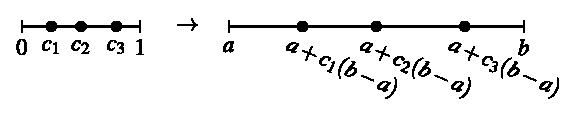
\includegraphics[width=0.4\linewidth]{kap4_1}
			\end{figure}
		
		
		\item \textbf{Nennen Sie einige einfache Quadraturformeln inklusive Knoten und Gewichte.}
			\begin{figure}[htbp]
				\centering
				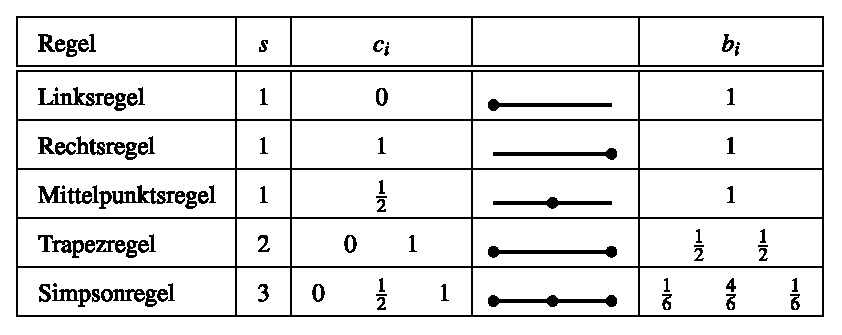
\includegraphics[width=0.6\linewidth]{kap4_2}
			\end{figure}
		
		\pagebreak
		
		\item \textbf{Erklären Sie den Begriff \textit{zusammengesetzte Quadraturformel}.} \\
			Ist der Abstand \(b-a\) sehr groß oder ändert sich der Integrand im Integrationsbereich \([a,b]\) rasch, zerlegt man \([a,b]\) in \(n\) Teilintervalle \([x_0,x_1],[x_1,x_2],\dots,[x_{n-1},x_n]\) mit \(a=x_0<x_1<x_2<\cdots<x_{n-1}<x_n=b\). Das Integral wird aufgespalten in eine Summe von \(n\) Teilintegralen über die einzelnen Teilintervalle:
			\begin{align*}
				\int_{a}^{b}f(x)\dif{x}=\int_{x_0}^{x_1}f(x)\dif{x}+\int_{x_1}^{x_2}f(x)\dif{x}+\cdots+\int_{x_{n-1}}^{x_n}f(x)\dif{x}
			\end{align*}
			Jedes dieser Teilintegrale \(\int_{x_{k-1}}^{x_k}f(x)\dif{x}\) wird mit einer Quadraturformel numerisch berechnet.\\
			Genauer Definiert mit der Definition aus 4.2: \\
			Es sei eine Quadraturformel \(Q=(b_i,c_i)^s_{i=1}\) und eine Unterteilung des Intervalls \([a,b]\) wie oben gegeben. Dann heißt eine Näherungsformel
			\begin{align*}
				\int_{a}^{b}f(x)\dif{x}\approx\sum_{k=1}^{n}Q(f,[x_{k-1}],x_k)=\sum_{k=1}^{n}h_k\sum_{i=1}^{s}b_if(x_{k-1}+c_ih_k)=:S_Q(f,x_0,\dots,x_n)
			\end{align*}
			mit \(h_k=x_k-x_{k-1}\) zusammengesetzte Quadraturformel oder Summe von Quadraturformeln. Für eine äquidistante Unterteilung von \([a,b]\) in \(n\) Teilintervalle, also
			\begin{align*}
				x_k=a+kh, \quad h=\frac{b-a}{n}, \quad k=0,\dots,n,
			\end{align*}
			haben wir folgende Näherungsformel
			\begin{align*}
				\int_{a}^{b}f(x)\dif{x}\approx h\sum_{k=1}^{n}\sum_{i=1}^{s}b_if(x_{k-1}+c_ih)=:S_Q(f,h,[a,b])=S_Q(f,h).
			\end{align*}
		
		\item \textbf{Wie erhält man Quadraturformeln mit Hilfe von Polynominterpolation?} \\
			
		
		\item \textbf{Erklären Sie den Begriff \textit{Ordnung} einer Quadraturformel. Wie bestimmt man die Ordnung?} \\
		
		\item \textbf{Was sind \textit{Bedingungsgleichungen}?} \\
		
		\item \textbf{Erklären Sie die Begriffe \textit{Fehler einer Quadraturformel} und \textit{Fehlerkonstante}.} \\
		
		\item \textbf{Was für Abschätzungen gelten für den Fehler einer Quadraturformel bzw. einer zusammengesetzten Quadraturformel? Was muss der Integrand $f$ dabei erfüllen?} \\
		
		\item \textbf{Was sind \textit{symmetrische Quadraturformeln} und welche Eigenschaft besitzen sie?} \\
		
		\item \textbf{Was ist eine Gaußsche Quadraturformel? Welche Ordnung besitzen sie?} \\
		
		\item \textbf{Wie groß kann die Ordnung einer Quadraturformel maximal sein?} \\
		
		\item \textbf{Was gilt für die Gewichte einer Gaußschen Quadraturformel?} \\
		
		\item \textbf{Wie funktioniert eine Schrittweitensteuerung? Erklären Sie die Begriffe \textit{Fehlerkriterium} und \textit{Fehlerschätzer}.} \\
		
		\item \textbf{Erklären Sie den Begriff \textit{Richardson-Extrapolation}. Wie berechnet man est und $\mathbf{Q_extr}$.} \\
		
		\item \textbf{Was passiert bei Integranden mit Singularitäten oder Singularitäten in den Ableitungen?} \\
		
		\item \textbf{Wie werden Doppelintegrale auf Rechtecken numerisch berechnet?} \\
		
		\item \textbf{Wie werden Doppelintegrale auf Dreiecken numerisch berechnet? Wie überprüft man die Ordnung einer Quadraturformel für Dreiecke?} \\
		
		\item \textbf{Was sind \textit{baryzentrische Koordinaten}?} \\
		
	\end{enumerate}
	\newpage
	% !TeX spellcheck = de_AT_frami
\section{Numerische Integration}
	\begin{enumerate}
		\item \textbf{Wie ist die LU-Zerlegung definiert?} \\
		
		\item \textbf{Was bedeutet Spaltenpivotsuche und wieso wird sie verwendet?} \\
		
		\item \textbf{Wie erhält man die Permutationsmatrix bzw. den Permutationsvektor?} \\
		
		\item \textbf{Wie löst man die LU-Zerlegung lineare Gleichungssysteme \(\mathbf{AX=b}\)?} \\
		
		\item \textbf{Wie berechnet man \(\mathbf{\det A}\) mit Hilfe der LU-Zerlegung?} \\
		
		\item \textbf{Wie groß ist der Rechenaufwand der LU-Zerlegung und für das Auflösen eines linearen Gleichungssystems?} \\
		
		\item \textbf{Wie ist die Cholesky-Zerlegung einer Matrix A definiert? Welche Eigenschaften muss A besitzen?} \\
		
		\item \textbf{Wie berechnet man die Cholesky-Zerlegung?} \\
		
		\item \textbf{Wie groß ist der Rechenaufwand einer Cholesky-Zerlegung?} \\
		
		\item \textbf{Wie löst man mit der Cholesky-Zerlegung lineare Gleichungssysteme \(\mathbf{AX=b}\)?} \\
		
		\item \textbf{Wie ist die rationale Cholesky-Zerlegung einer Matrix A definiert? Welche Eigenschaften muss A besitzen?} \\
		
		\item \textbf{Wie berechnet man die rationale Cholesky-Zerlegung?} \\
		
		\item \textbf{Wie löst man mit der rationalen Cholesky-Zerlegung lineare Gleichungssysteme \(\mathbf{AX=b}\)?} \\
		
		\item \textbf{Wie ist die Matrixnorm allgemein definiert?} \\
		
		\item \textbf{Wie berechnet man \(\mathbf{||\text{A}||_1}\), \(\mathbf{||\text{A}||_2}\) und \(\mathbf{||\text{A}||_\infty}\) ?} \\
		
		\item \textbf{Wie ist die Norm von \(\mathbf{A^{-1}}\) definiert?} \\
		
		\item \textbf{Wie ist die Kondition einer linear Abbildung bzw. einer Matrix A definiert?} \\
		
		\item \textbf{Was gilt für den relativen Fehler der Lösung eines linearen Gleichungssystems?} \\
		
		\item \textbf{Welche Eigenschaften besitzt die Kondition einer Matrix?} \\
		
		\item \textbf{Welche Matrizen haben eine große/kleine Kondition?} \\
		
		\item \textbf{Was ist die Kondition der Einheitsmatrix?} \\
		
		\item \textbf{Wie lässt sich die Kondition einer Matrix geometrisch interpretieren?} \\
		
		\item \textbf{Wie lässt sich die Kondition eines linearen Gleichungssystems geometrisch interpretieren?} \\
		
		\item \textbf{Wie ist die QR-Zerlegung definiert? Wozu wird sie verwendet?} \\
		
	\end{enumerate}
	\newpage
	% !TeX spellcheck = de_AT_frami
\section{Numerische Integration}
	\begin{enumerate}
		\item \textbf{Beschreiben Sie das Newton-Verfahren in einer Veränderlichen. Skizze!} \\
		
		\item \textbf{Wie ist das Newton-Verfahren in mehreren Veränderlichen definiert?} \\
		
		\item \textbf{Wie schnell konvergiert das Newton-Verfahren? Welche Voraussetzungen muss der Startwert erfüllen?} \\
		
		\item \textbf{Wie ist das Gauß-Newton-Verfahren definiert?} \\
		
		\item \textbf{Wie ist das Konvergenzverhalten des Gauß-Newton-Verfahrens?} \\
		
	\end{enumerate}
	\newpage
	% !TeX spellcheck = de_AT_frami
\section{Ausgleichsrechnung und Approximation}
	\begin{enumerate}
		\item \textbf{Was bedeutet der Begriff \textit{Methode der kleinsten Fehlerquadrate}?} \\
			Die Summe der Fehlerquadrate
			\begin{align*}
				\sum_{i=0}^{m}(f(x_i)-y_i)^2
			\end{align*}
			soll minimal sein.
		\item \textbf{Was sind Gründe eine Funktion oder ein Polynom nicht direkt durch die Punkte hindurch zu legen, sondern dazwischen hindurch?} \\
			Die Werte \(y_i\) sind mit Fehlern behaftet (Rundungsfehler, Messfehler, Modellfehler). Zudem sind meist mehr Datenpunkte gegeben, als für eine eindeutige Bestimmung der Modellparameter \(a\)  der Modellfunktion \(f\) notwendig sind. Somit gibt es im Allgemeinen keine Modellfunktion \(f\), die exakt durch sämtliche Datenpunkte hindurchpasst.
		
		\item \textbf{Was bedeutet der Begriff \textit{Modellfunktion}?} \\
			Die Modellfunktion
			\begin{align*}
				f:\mathbb{R}^d\times\mathbb{R}^{n+1}\rightarrow\mathbb{R}:y=f(x_1,\dots,x_d,a_0,\dots,a_n)=f(x,a_0,\dots,a_n)
			\end{align*}
			hängt von den Inputdaten \(x=(x_1,\dots,x_d)\) und von sogenannten Modellparametern \(a=(a_0,\dots,a_n)\) ab und ist eine (möglichst einfache) Funktion, die den Zusammenhang zwischen den Inputdaten \(x_i\) und den Outputdaten \(y_i\) beschreiben soll.
		
		\item \textbf{Erklären Sie den Begriff \textit{lineare Ausgleichsrechnung}. Wie lässt sich hier die Modellfunktion schreiben?} \\
			Bei einer linearen Ausgleichsrechnung hängt die Modellfunktion \(f\) für festes \(x\) nur linear von den Modellparametern \(a_0,\dots,a_n\) ab. Dadurch lässt sich \(f\) als Linearkombination aus linear unabhängigen (aber nicht unbedingt linearen) Funktionen \(f_0,\dots,f_n\) schreiben.
			\begin{align*}
				\text{Fa}=\text{y}
			\end{align*}
			Sollte \(f\) linear unabhängig sein, kann man obige Gleichung im Sinne der kleinsten Fehlerquadrate gelöst werden.
			\begin{align*}
				\text{Suche } a_0,\dots,a_n,\text{ sodass } ||\text{Fa-y}||^2=\sum_{i=0}^{m}\left(F_{i*}a-y_i\right)^ \text{minimal.}
			\end{align*}
		
		\item \textbf{Erklären Sie den Begriff \textit{nichtlineare Ausgleichsrechnung}.} \\
			Bei einer nichtlinearen Ausgleichsrechnung hängt die  Modellfunktion \(f\) für festes \(x\) nichtlinear von den Modellparametern \(a_0,\dots,a_n \) ab. Setzt man die Datenpunkte \((x_0,y_0),\dots,(x_m,y_m)\) in die Modellfunktion ein erhält man ein überbestimmtes, nichtlineares Gleichungssystem
			\begin{align*}
				f(x_0,a_0,\dots,a_n)-y_0 & =0     \\
				f(x_1,a_0,\dots,a_n)-y_1 & =0     \\
				                        & \hspace{0.16cm}\vdots \\
				f(x_m,a_0,\dots,a_n)-y_m & =0
			\end{align*}
		
		\item \textbf{Worin besteht der Unterschied zwischen \textit{linearer} und \textit{nichtlinearer Ausgleichsrechnung}?} \\
			In der linearen/nichlinearen Abhängigkeit der Modellfunktion \(f\) von den Modellparametern \(a_0,\dots,a_n\).
		
		\item \textbf{Sie legen eine Ausgleichsparabel zwischen den Punkten hindurch. Ist dies lineare oder	nichtlineare Ausgleichsrechnung?} \\
			linear
		
		\item \textbf{Welche zwei gegensätzlichen Ziele werden bei den \textit{glättenden Splines} betrachtet bzw. optimiert?}
			\begin{enumerate}
				\item[(1)] Die Splinefunktion \(s\) soll "möglichst gut" zwischen den Datenpunkten hindurchpassen. \\
							D.h. es soll die Summe \(\sum_{i=0}^{n}\left(y_i-s(x_i)\right)^2\) der Fehlerquadrate möglichst klein sein.
				\item[(2)] Die Splinefunktion \(s\) soll "möglichst glatt" sein, d.h. die potentielle Energie bzw. die Gesamtkrümmung bzw. das Integral \(\int_{x_0}^{x_n}\left(s''(x)\right)^2\) soll möglichst klein sein.
			\end{enumerate}
		
		\item \textbf{Was bedeutet ein Wert des \textit{Glättungsparameters} \(\mathbf{\lambda}\) nahe 0 bzw. nahe 1?} \\
			Obige widersprüchliche Ziele werden zum Optimierungsproblem
			\begin{align*}
				\lambda\cdot\sum_{i=0}^{n}\left(y_i-s(x_i)\right)^2+\left(1-\lambda\right)\cdot\int_{x_0}^{x_n}\left(s''(x)\right)^2 \rightarrow \text{ min,} \quad \lambda\in(0,1]
			\end{align*}
			Verknüpft, wobei \(\lambda\) zwischen ihnen Gewichtet.
			\begin{itemize}
				\item \(\lambda\) nahe bei 0 bedeutet, dass die Glattheit des Splines sehr wichtig ist.
				\item \(\lambda\) nahe bei 1 bedeutet, dass kleine Fehlerquadrate wichtiger sind.
			\end{itemize}
			Man wählt also zwischen \(s\rightarrow\)Ausgleichsgerade für \(\lambda\rightarrow 0\) und ungeglätteten Spline für \(\lambda \rightarrow 1\).
		
		\item \textbf{Was passiert, wenn man \(\mathbf{\lambda=1}\) nimmt?} \\
			Bei \(\lambda=0\) wäre jede Funktion \(s\) mit \(s''=0\) Lösung des Optimierungsproblems, da dann der Fehler völlig egal wäre. Daher wird der Fall nicht betrachtet.\\
			Allerdings gilt: \(s\rightarrow\)Ausgleichsgerade für \(\lambda\rightarrow 0\).
		
		\item \textbf{Was passiert, wenn man \(\mathbf{\lambda}\) gegen 0 gehen lässt?} \\
			Bei \(\lambda=1\) ist die potentielle Energie bzw. Glattheit egal und nur die Fehlerquadrate wichtig. In diesem Fall erhalten wir wieder den üblichen Spline, der exakt durch die Datenpunkte geht.
	\end{enumerate}
	\newpage
	% !TeX spellcheck = de_AT_frami
\section{Gewöhnliche Differentialgleichungen}
	\begin{enumerate}
		\item \textbf{Beschreiben Sie das \textit{explizite Euler-Verfahren} einer Dimension. Skizze!}
		\item \textbf{Wie schreibt man ein System von Differentialgleichungen zweiter Ordnung in ein System erster Ordnung um?}
		\item \textbf{Erklären Sie die Begriffe \textit{Runge-Kutta-Verfahren} und \textit{Butcher-Tableau}.}
		\item \textbf{Wie ist die Ordnung \(\mathbf{p}\) eines numerischen Verfahrens zur Lösung von Differentialgleichungen definiert?}
		\item \textbf{Was gilt für den \textit{lokalen} bzw. \textit{globalen Fehler} bei einem Verfahren mit Ordnung \(\mathbf{p}\)?}
		\item \textbf{Wie lässt sich die Ordnung \(\mathbf{p}\) experimentell feststellen?}
		\item \textbf{Was bedeutet der Begriff \textit{steife Differentialgleichung}?}
		\item \textbf{Es sei die Differentialgleichung \(\mathbf{y′=−200y, y(0)=1}\), gegeben. Wie groß darf man die Schrittweite \(\mathbf{h}\) maximal wählen, damit die numerische Lösung stabil bleibt, d.h. im Bereich zwischen −1 und 1 bleibt?}
		\item \textbf{Wie lässt sich der \textit{Fehler} \texttt{est} bei einer Schrittweitensteuerung schätzen?}
		\item \textbf{Wie bestimmt man bei einer Schrittweitensteuerung die \textit{optimale Schrittweite} \(\mathbf{h}_\texttt{opt}\)?}
	\end{enumerate}	
\end{document}